%%%%%%%%%%%%%%%%%%%%%%%%%%%%%%%%%%%%%%%%%
% Contract LaTeX Template Version 1.0 (December 8 2014)
%
% This template has been downloaded from: http://www.LaTeXTemplates.com
%
% Original author: Brandon Fryslie With extensive modifications by: Vel
% (vel@latextemplates.com)
%
% License: CC BY-NC-SA 3.0 (http://creativecommons.org/licenses/by-nc-sa/3.0/)
%
% Authors: Sabbir Ahmed, Jeffrey Osazuwa, Howard To, Brian Weber
% 
%%%%%%%%%%%%%%%%%%%%%%%%%%%%%%%%%%%%%%%%%

\documentclass[paper=usletter, fontsize=12pt]{article}
\usepackage{graphicx}
%%%%%%%%%%%%%%%%%%%%%%%%%%%%%%%%%%%%%%%%%
% Contract
% Structural Definitions File
% Version 1.0 (December 8 2014)
%
% Created by:
% Vel (vel@latextemplates.com)
% 
% This file has been downloaded from:
% http://www.LaTeXTemplates.com
%
% License:
% CC BY-NC-SA 3.0 (http://creativecommons.org/licenses/by-nc-sa/3.0/)
%
%%%%%%%%%%%%%%%%%%%%%%%%%%%%%%%%%%%%%%%%%

%----------------------------------------------------------------------------------------
%   PARAGRAPH SPACING SPECIFICATIONS
%----------------------------------------------------------------------------------------

\setlength{\parindent}{0mm} % Don't indent paragraphs

\setlength{\parskip}{2.5mm} % Whitespace between paragraphs

%----------------------------------------------------------------------------------------
%   PAGE LAYOUT SPECIFICATIONS
%----------------------------------------------------------------------------------------

\usepackage{geometry} % Required to modify the page layout
\usepackage{multicol}

\setlength{\textwidth}{16cm} % Width of the text on the page
\setlength{\textheight}{23cm} % Height of the text on the page

\setlength{\oddsidemargin}{0cm} % Width of the margin - negative to move text left, positive to move it right

% Uncomment for offset margins if the 'twoside' document class option is used
%\setlength{\evensidemargin}{-0.75cm} 
%\setlength{\oddsidemargin}{0.75cm}

\setlength{\topmargin}{-1.25cm} % Reduce the top margin

%-------------------------------------------

\usepackage[utf8]{inputenc} % Required for including letters with accents
\usepackage[T1]{fontenc} % Use 8-bit encoding that has 256 glyphs

\usepackage{avant} % Use the Avantgarde font for headings
\usepackage{mathptmx} % Use the Adobe Times Roman as the default text font together with math symbols from the Sym­bol, Chancery and Com­puter Modern fonts

%----------------------------------------------------------------------------------------
%   SECTION TITLE SPECIFICATIONS
%----------------------------------------------------------------------------------------

\usepackage{titlesec} % Required for modifying section titles

\titleformat{\section} % Customize the \section{} section title
{\sffamily\large\bfseries} % Title font customizations
{\thesection} % Section number
{16pt} % Whitespace between the number and title
{\large} % Title font size
\titlespacing*{\section}{0mm}{7mm}{0mm} % Left, top and bottom spacing around the title

\titleformat{\subsection} % Customize the \subsection{} section title
{\sffamily\normalsize\bfseries} % Title font customizations
{\thesubsection} % Subsection number
{16pt} % Whitespace between the number and title
{\normalsize} % Title font size
\titlespacing*{\subsection}{0mm}{5mm}{0mm} % Left, top and bottom spacing around the title
\renewcommand\familydefault{\sfdefault} % specifies the document layout and style

\newcommand{\team}{Galois Field Arithmetic Unit}
\newcommand{\Sabbir}{Sabbir Ahmed}
\newcommand{\Jeffrey}{Jeffrey Osazuwa}
\newcommand{\Howard}{Howard To}
\newcommand{\Brian}{Brian Weber}

%----------------------------------------------------------------------------------------

% document info command
\newcommand{\documentinfo}[5]{
    \begin{centering}
        \parbox{6.8in}{
        \begin{spacing}{1}
            \begin{flushleft}
                \begin{tabular}{l l} #1 \\ #2 \\ #3 \\ #4 \\ #5 \\
                \end{tabular} \\
                \rule{\textwidth}{1pt}
            \end{flushleft}
        \end{spacing} }
    \end{centering} }

\begin{document}

    \documentinfo{\textbf{MEMO:} TSR-06}{\textbf{DATE: }{\today}}{\textbf{TO: }
    EFC LaBerge}{\textbf{FROM: }\Sabbir, \Jeffrey, \Howard,
    \Brian}{\textbf{SUBJECT: } Team Status Report}
    \vspace{-0.3in}

    \section{Introduction} The Galois Field Arithmetic Unit will accept two inputs
    a and b and determine the desired arithmetic result n, and to establish the field generating polynomial. The unit would serve as a computation engine for a relatively low-powered
    microcontroller, and would enable complex code and encryption algorithms.
    Project will include implementation of a Reed Solomon encoder and decoder
    using the GFAU. The purpose of this report is to detail the progress of the
    GFAU in the period of December 7, 2017 through February 9, 2018. This is
    the sixth and first status report for the second semester for the GFAU
    team.

    \section{Completed Tasks} During this work period, the team has continued
    to make progress on the GFAU. Including the following achievements:
    \begin{enumerate}[label=\alph*)]

        \item Most VHDL coding is done with issues detail in the Current Issues section of this document. 
        \item Updated system block diagram (see Figure 1 below). 
        \item Completed breakout board design. 
        
    \end{enumerate}

    \section{Planned Tasks}
   
    \begin{enumerate}[label=\alph*)]

        \item Order breakout board.
        \item Program FPGA with VHDL code and resolve any issues arise. 
        \item Interface FPGA with external memory.

    \end{enumerate}

    \section{Current Issues} Current issues the team are having include: 
	
	\begin{enumerate}[label=\alph*)]
		\item Need to receive testing instruments from Dr. LaBerge to verify design. 
		\item Timing issue with zero and the zeroth term and their memory address.
		\item Timing issue with generating polynomials.		
		\item Problem generating one symbol per clock cycle.
		\item Not sure how to simulate memory and IO with VHDL.
	\end{enumerate}
	
	%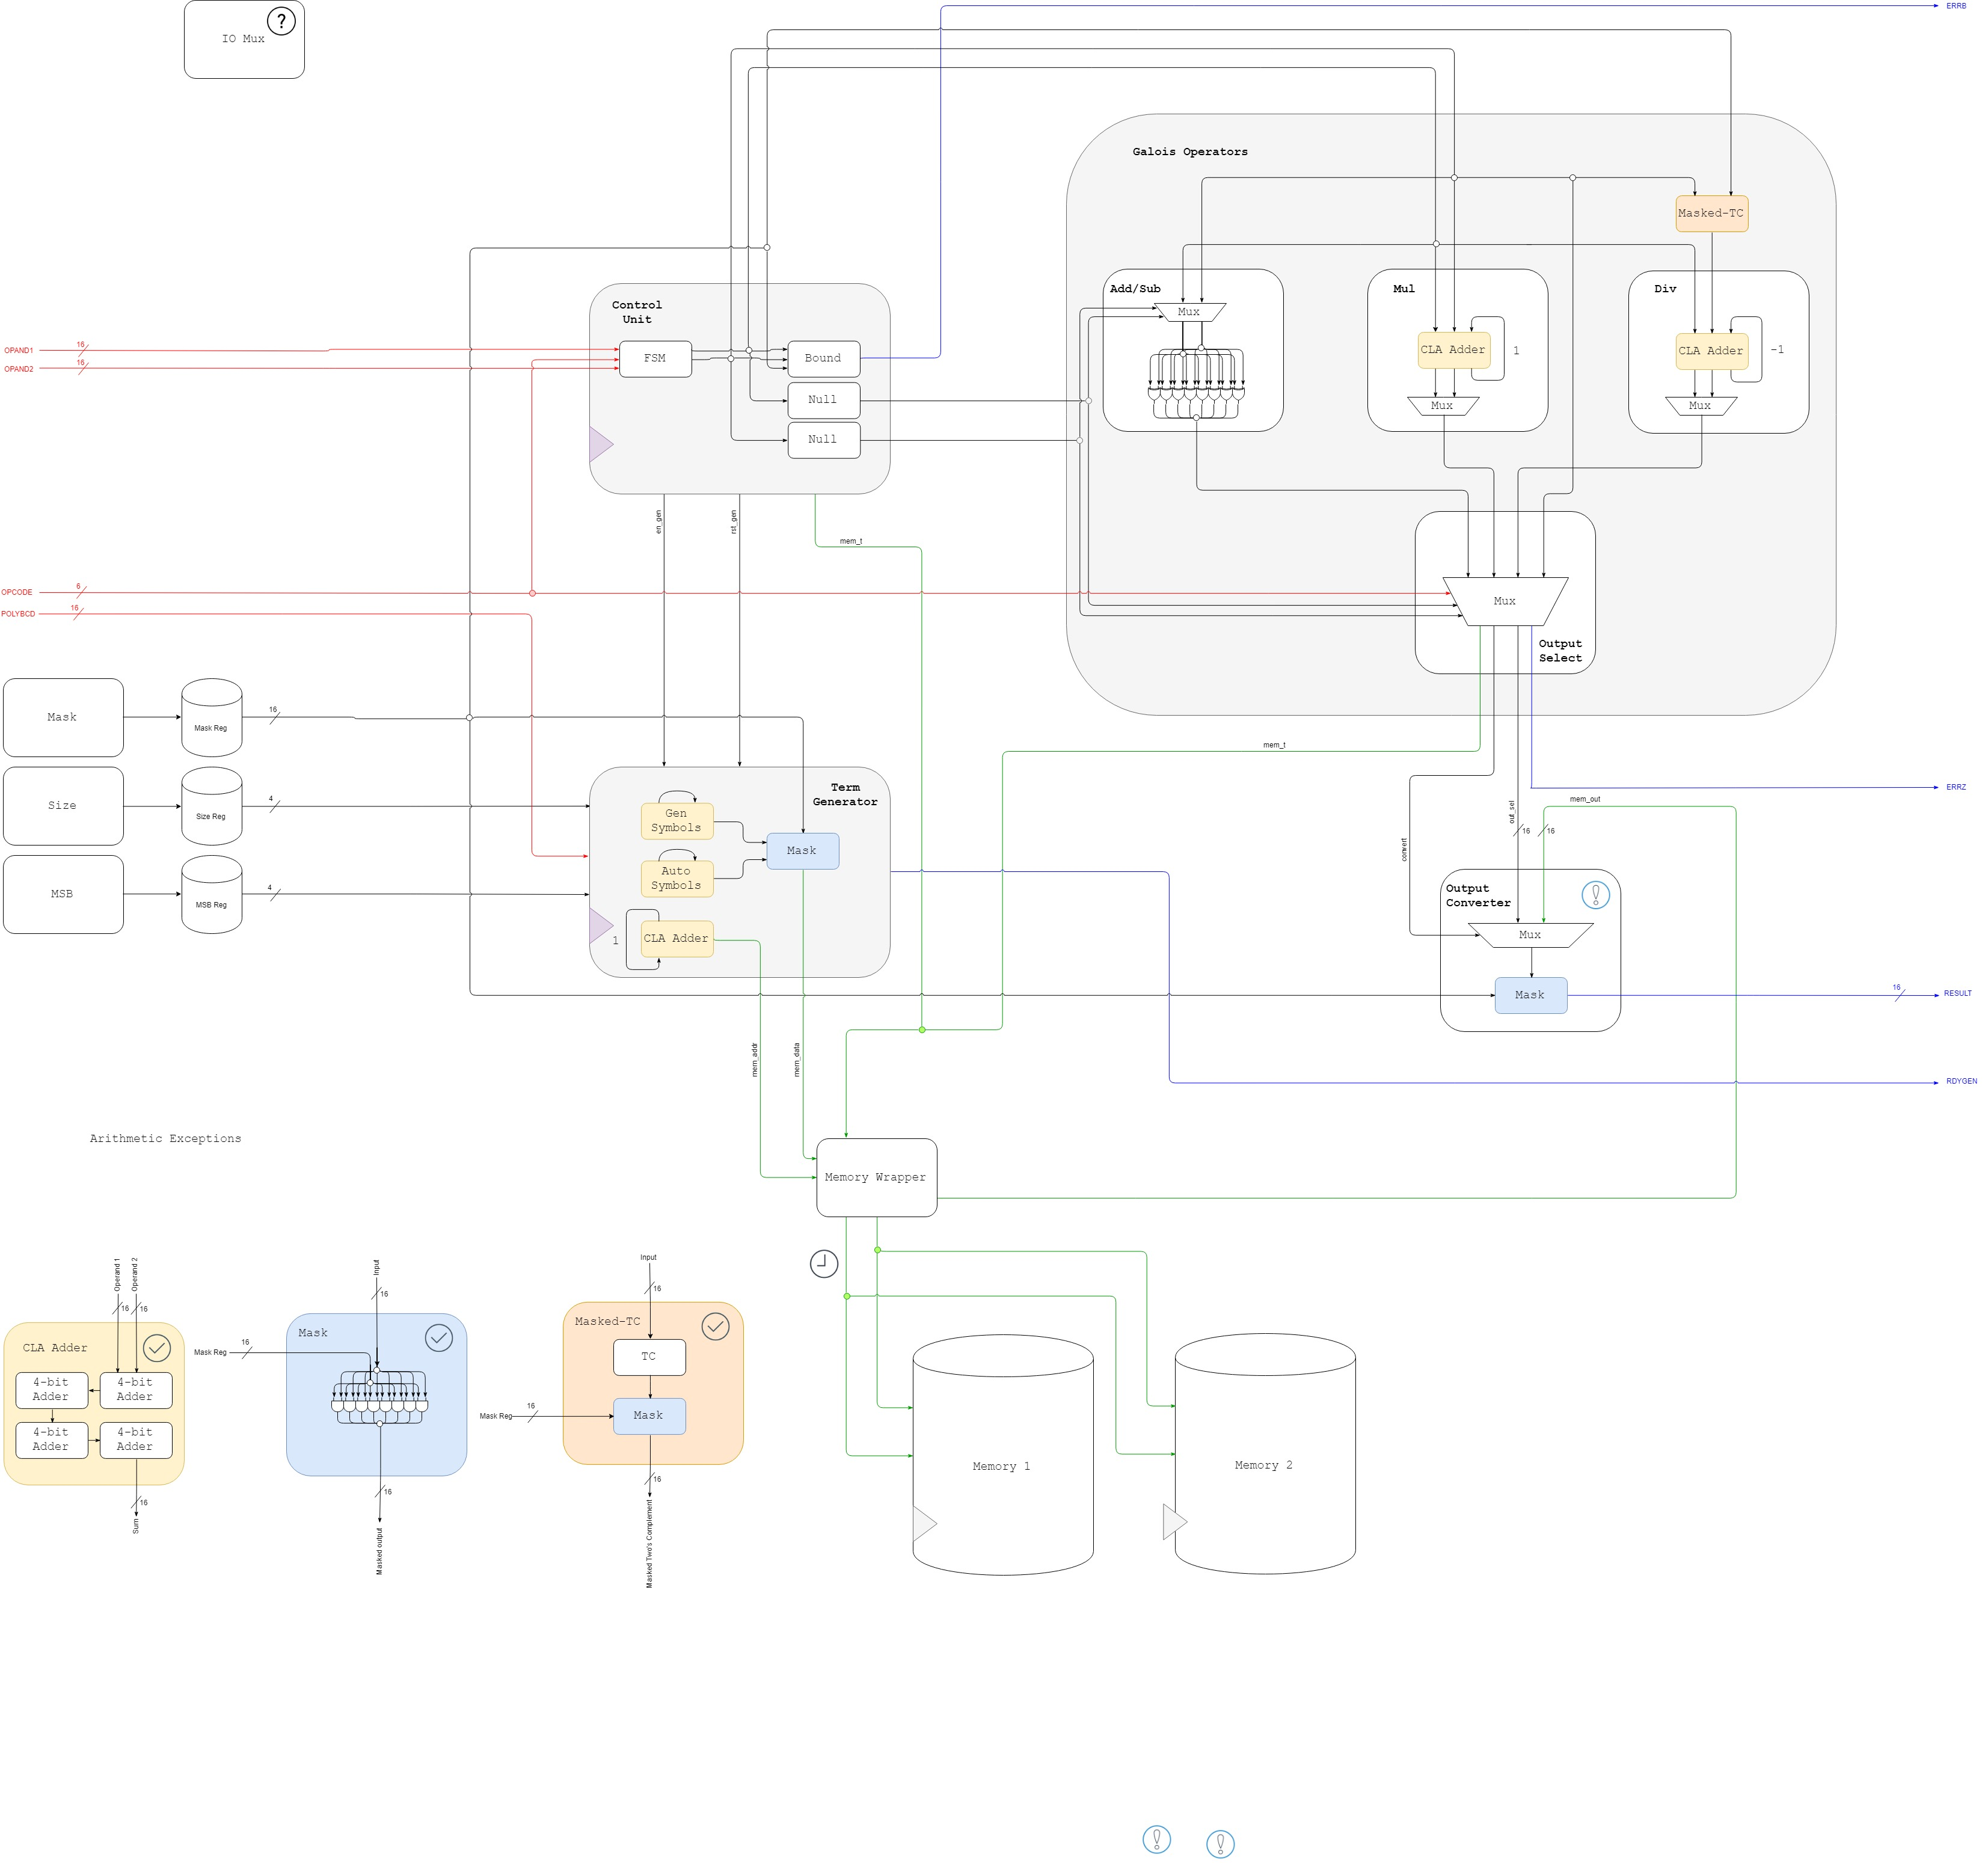
\includegraphics[scale=0.17]{system_block_diagram}
  	\begin{figure}[h!]
  		
  		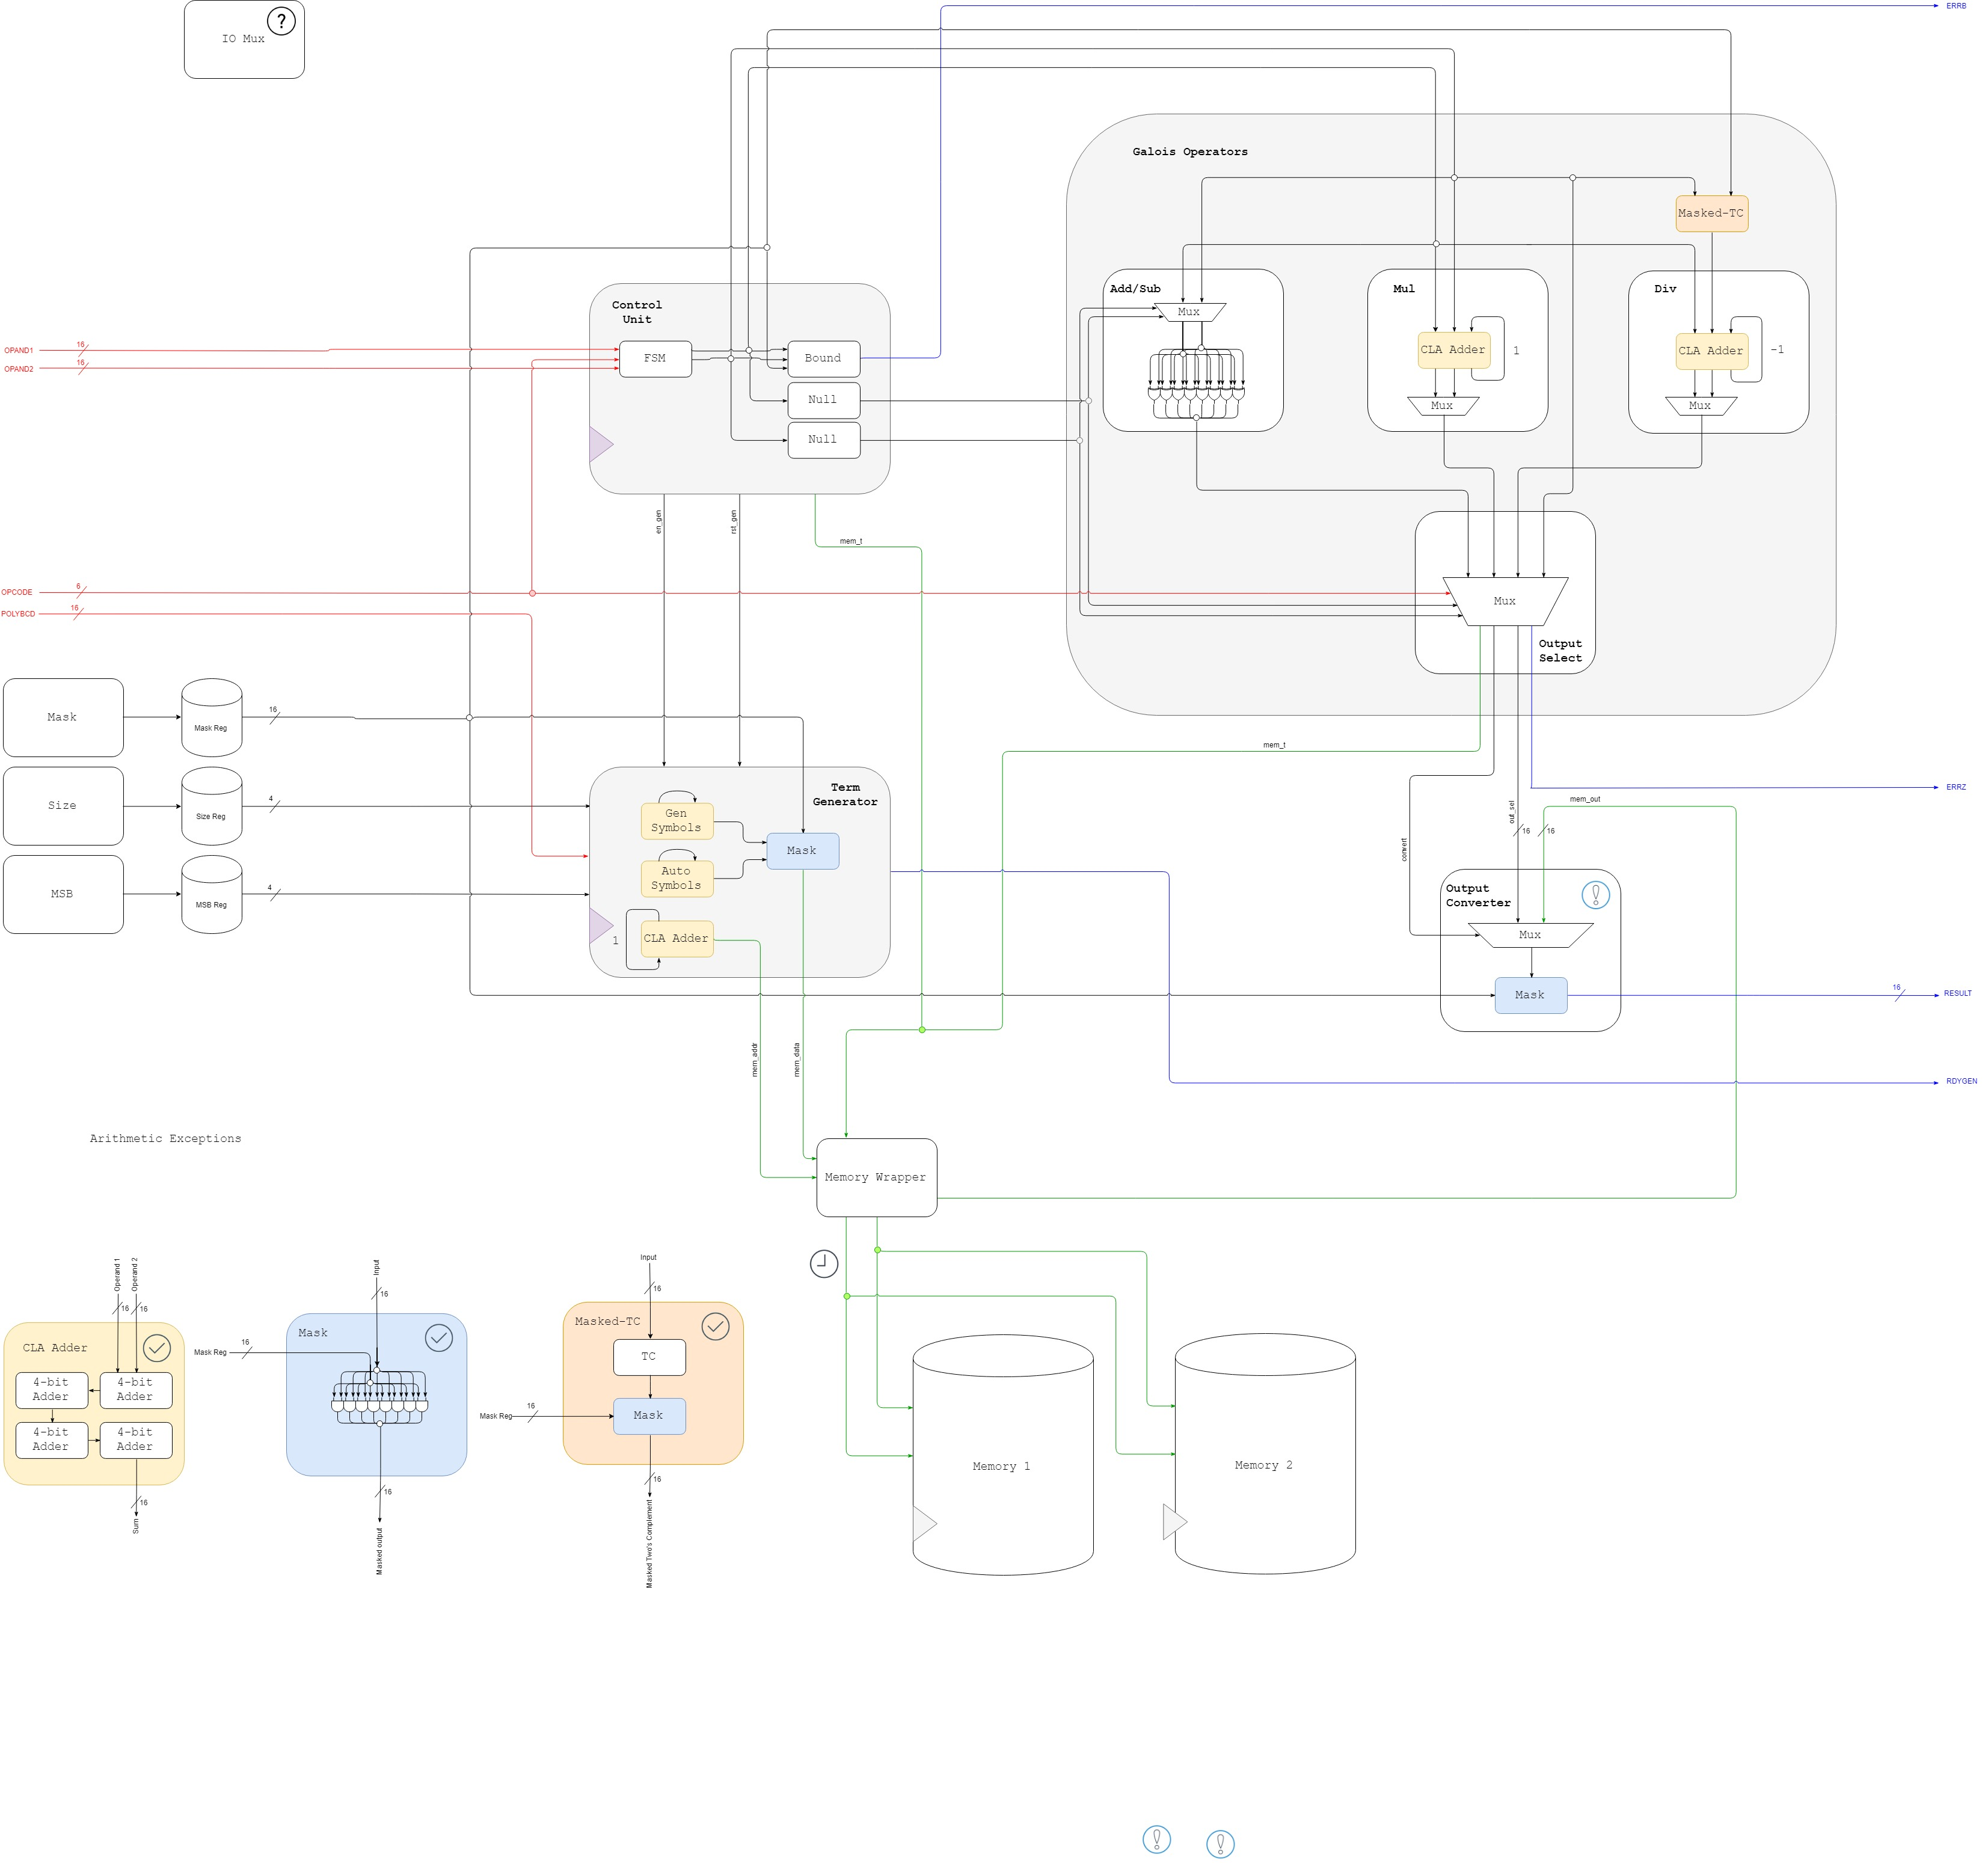
\includegraphics[scale=0.16]{system_block_diagram}
  		\caption{System block diagram}
  	\end{figure}
   
   
\end{document}
